
\section{9600-Port}
\label{section:9600_port}
\begin{frame}%STARTCONTENT
\begin{itemize}
  \item Zur Umgehung von Filtern bieten manche FM-Funkgeräte einen separaten Port für Digimodes
  \item Dieser ist oft mit \emph{DATA} oder \emph{9600} beschriftet
  \item 9600 entsprechend der Datenrate in Baud, die damit übertragen werden kann
  \item Daran wird direkt das TNC (Terminal Node Controller) vom Computer angeschlossen
  \item Heute oft direkt als USB-Anschluss ausgeführt
  \end{itemize}
\end{frame}

\begin{frame}
\begin{columns}
    \begin{column}{0.48\textwidth}
    \begin{itemize}
  \item Sowohl Senden als auch Empfang findet ohne NF-Filter und NF-Endstufe statt
  \item Es wird direkt der FM-Modulator oder FM-Demodulator angesprochen
  \item Signale werden nicht verzerrt
  \end{itemize}

    \end{column}
   \begin{column}{0.48\textwidth}
       
\begin{figure}
    \DARCimage{0.85\linewidth}{354include}
    \caption{\scriptsize FM-Sender mit Zuführung des 9600-Baud-Datensignals an Punkt 2}
    \label{e_9600_port_fm_sender}
\end{figure}


\begin{figure}
    \DARCimage{0.85\linewidth}{355include}
    \caption{\scriptsize FM-Empfänger mit Abgreifen des 9600-Baud-Datensignals an Punkt 4}
    \label{e_9600_port_fm_empfaenger}
\end{figure}


   \end{column}
\end{columns}

\end{frame}

\begin{frame}
\begin{columns}
    \begin{column}{0.48\textwidth}
    \begin{itemize}
  \item Wurde früher für Packet Radio verwendet
  \item Heute für moderne und freie Modi wie M17
  \end{itemize}

    \end{column}
   \begin{column}{0.48\textwidth}
       
\begin{figure}
    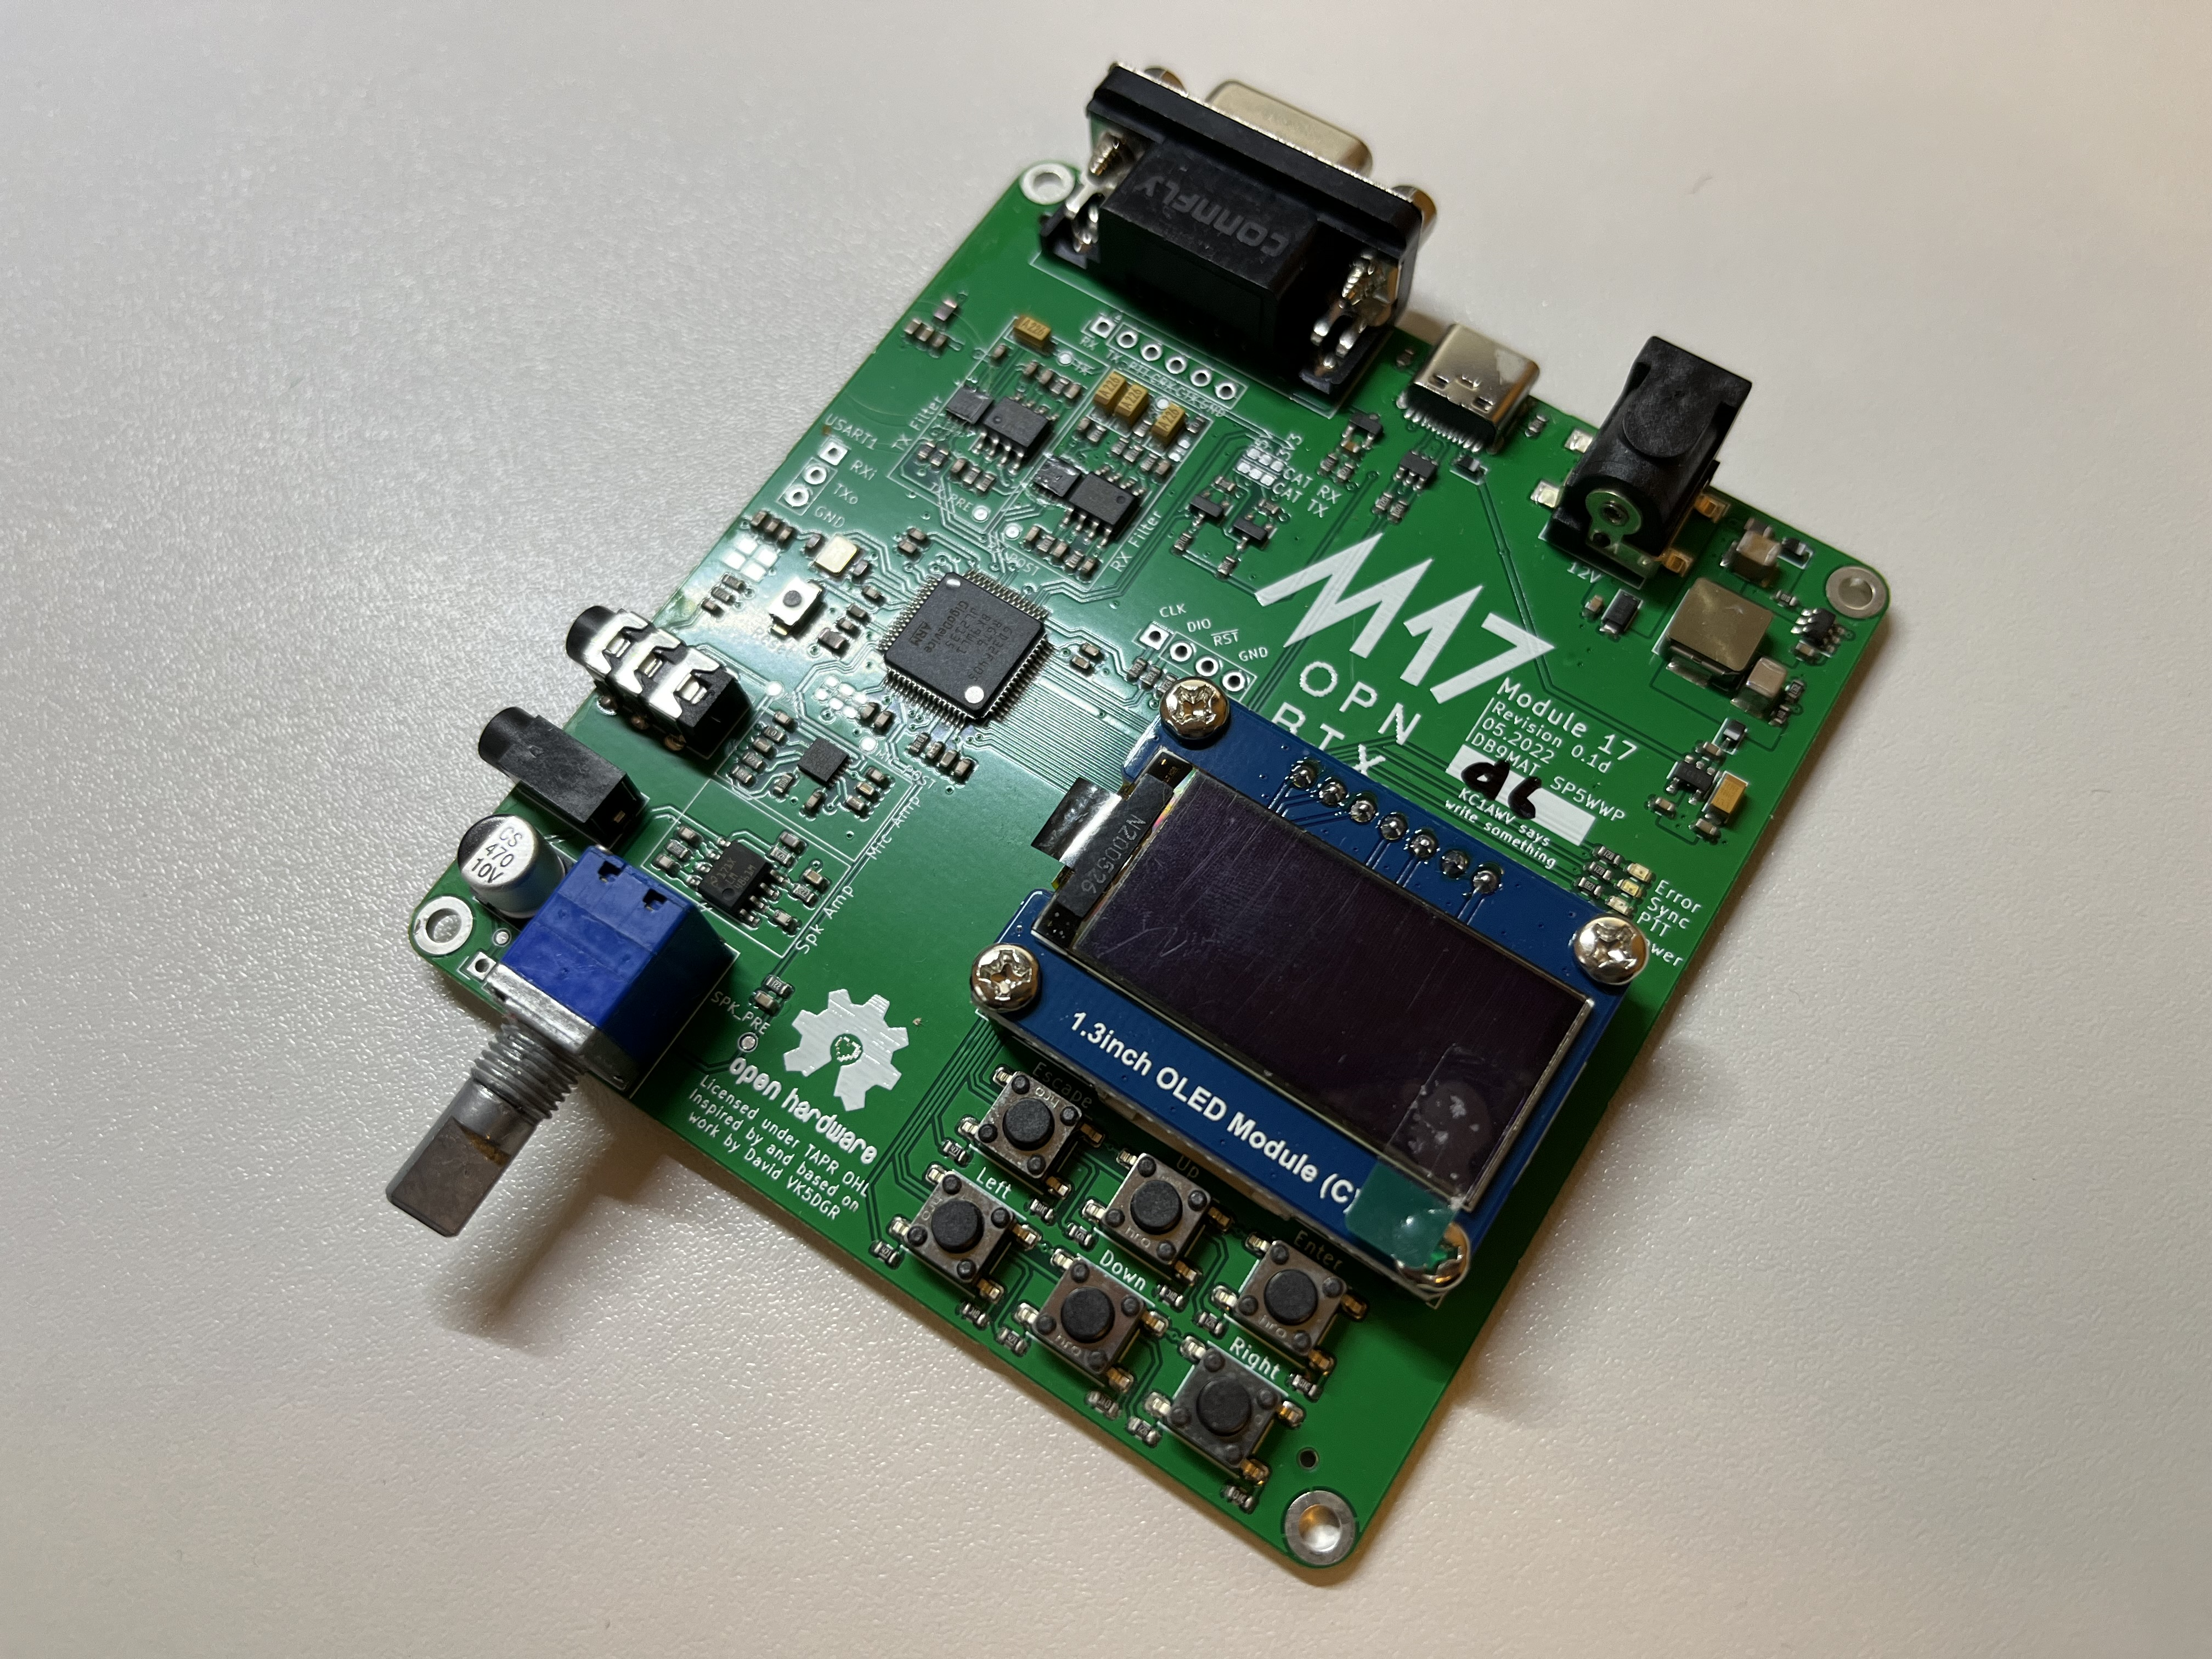
\includegraphics[width=0.85\textwidth]{foto/185}
    \caption{\scriptsize Module M17 ein TNC für das M17 Übertragungsverfahren}
    \label{m17_tnc}
\end{figure}

   \end{column}
\end{columns}

\end{frame}

\begin{frame}
\only<1>{
\begin{PQuestion}{EF309}{Welcher der eingezeichneten Punkte in einem FM-Sender ist für die Zuführung eines 9600-Baud-Datensignals am besten geeignet?}{Punkt 2}
{Punkt 1}
{Punkt 3}
{Punkt 4}
{\DARCimage{1.0\linewidth}{354include}}\end{PQuestion}

}
\only<2>{
\begin{PQuestion}{EF309}{Welcher der eingezeichneten Punkte in einem FM-Sender ist für die Zuführung eines 9600-Baud-Datensignals am besten geeignet?}{\textbf{\textcolor{DARCgreen}{Punkt 2}}}
{Punkt 1}
{Punkt 3}
{Punkt 4}
{\DARCimage{1.0\linewidth}{354include}}\end{PQuestion}

}
\end{frame}

\begin{frame}
\only<1>{
\begin{PQuestion}{EF219}{Manche FM-Transceiver verfügen über einen analogen Datenanschluss (z.~B. mit DATA beschriftet oder als 9600-Port bezeichnet). Welcher Punkt im dargestellten Empfangszweig wird über diesen Anschluss üblicherweise herausgeführt?}{Punkt 1}
{Punkt 4}
{Punkt 2}
{Punkt 3}
{\DARCimage{1.0\linewidth}{355include}}\end{PQuestion}

}
\only<2>{
\begin{PQuestion}{EF219}{Manche FM-Transceiver verfügen über einen analogen Datenanschluss (z.~B. mit DATA beschriftet oder als 9600-Port bezeichnet). Welcher Punkt im dargestellten Empfangszweig wird über diesen Anschluss üblicherweise herausgeführt?}{Punkt 1}
{\textbf{\textcolor{DARCgreen}{Punkt 4}}}
{Punkt 2}
{Punkt 3}
{\DARCimage{1.0\linewidth}{355include}}\end{PQuestion}

}
\end{frame}%ENDCONTENT
